\section{Tree-Parzen Estimator}
%-----------------------------------------------------------------------
%-----------------------------------------------------------------------
\begin{frame}[c]{Connection TPE-grey-box}

\comment{What should be the motivation for including TPE here? Just as an alternative for BO?}    

\end{frame}
%-----------------------------------------------------------------------
%-----------------------------------------------------------------------
\begin{frame}[c]{Tree-Parzen Estimator}

\begin{itemize}
	\item Assume that we already observed some configuration and the corresponding loss $D = \{(\conf_i, \boobs_i))\}_{i=1}^N$
	\begin{itemize}
		\item let's use $\boobs_i = f(\lambda)$ as a short form for $\mathcal{L}(\algo_{\conf}, \dataset_{train}, \dataset_{valid})$
	\end{itemize}
	\pause
	\item We could approximate the good and the bad regions of the configuration space $\pcs$
\end{itemize}

$$
p(\conf|y) = \begin{cases}
l(\conf) \text{ if } \boobs < \boobs^*\\
g(\conf) \text{ otherwise} 
\end{cases}
$$

where 
\begin{itemize}
	\item $\boobs^*$ is an empirical threshold for a well-performing configuration\\ (e.g., a $\gamma$ percentile of all observed $\boobs$ in $D$)
	\pause
	\item $l(\conf)$ models the density of the well-performing region based on $D$
\note[item] Note that we minimize!
	\pause
	\item $g(\conf)$ models the density of the poorly performing region based on $D$
	\pause
	\item $g$ and $l$ can be modeled by kernel density estimator (KDE)
\end{itemize}

\source{Bergstra et al. 2011}

\end{frame}
%-----------------------------------------------------------------------
%-----------------------------------------------------------------------
\begin{frame}[c]{Optimization with Tree-Parzen Estimator}
\begin{center}
\begin{minipage}{0.75\textwidth}
\begin{algorithm}[H]
    \LinesNumbered
    \SetAlgoLined
    \setcounter{AlgoLine}{0}
	\Input{Configuration Space $\pcs$,
		black box function $f$,
		maximal number of function evaluations $m$,
		percentile $\gamma$
	}
	\BlankLine
	$D_0$ $\leftarrow$ initial\_design($\pcs$); 
	\pause
	
	\For{\bocount = $1, 2, \ldots \bobudget - |\dataset_0|$}{
		$\dataset_\text{good}, \dataset_\text{bad}$ $\leftarrow$ Split $\dataset_{\bocount-1}$ into good and bad observations according to $\gamma$ percentile of all observed $\boobs$;
		\pause
		
		$l(\conf)$ $\leftarrow$ fit KDE on $\dataset_\text{good}$; 
		$g(\conf)$ $\leftarrow$ fit KDE on $\dataset_\text{bad}$;
		\pause
		
		$\Lambda_\text{cand}$ $\leftarrow$ draw examples according to $l$;
		\pause
		
		select $\conf_{\bocount}$ by optimizing $\conf_{\bocount} \in \argmax_{\conf \in \Lambda_\text{cand}} l(\conf) / g(\conf)$;
		\pause
		
		Query $\boobs_{\bocount} := \func(\lambda_{\bocount})$;
		
		Add observation to data $\dataset_{\bocount} := \dataset_{\bocount-1} \cup \{\langle \conf_{\bocount}, \boobs_{\bocount} \rangle \}$;
	}
	\Return{Best observed $\lambda$ according to $\dataset_\bobudget$}
	\caption{Optimization with TPE}
\end{algorithm}
\end{minipage}
\end{center}

\source{Bergstra et al. 2011}

\end{frame}
%-----------------------------------------------------------------------
%-----------------------------------------------------------------------
\begin{frame}[c]{Optimization with Tree-Parzen Estimator}

\centering
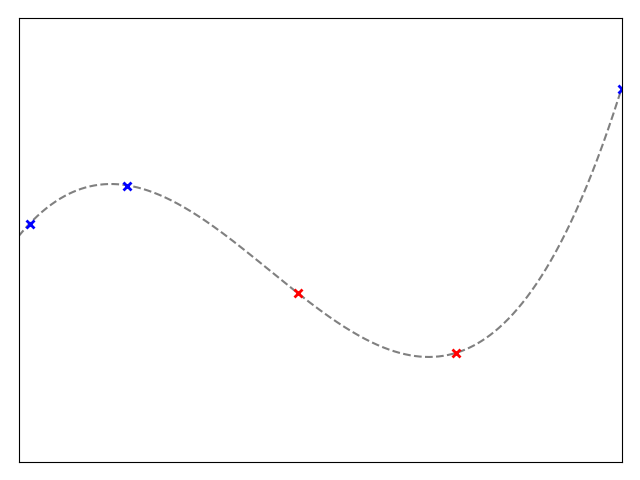
\includegraphics[width=0.6\textwidth]{w07_hpo_grey_box/images/tpe/tpeiter_1_observations.png}


\end{frame}
%-----------------------------------------------------------------------
%-----------------------------------------------------------------------
\begin{frame}[c]{Optimization with Tree-Parzen Estimator}

\centering
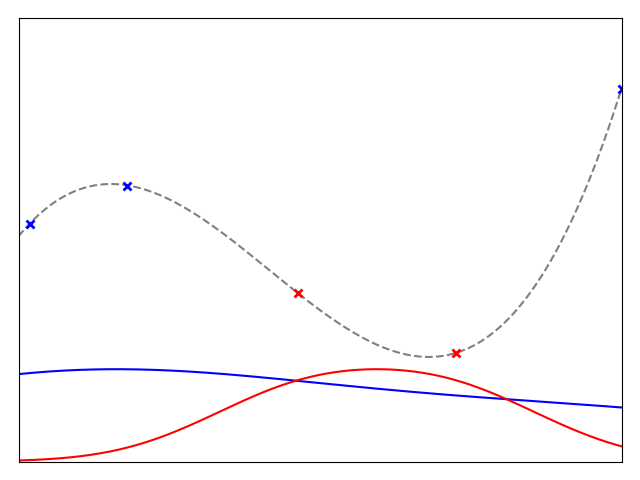
\includegraphics[width=0.6\textwidth]{w07_hpo_grey_box/images/tpe/tpeiter_1_pdfs.png}


\end{frame}
%-----------------------------------------------------------------------
%-----------------------------------------------------------------------
\begin{frame}[c]{Optimization with Tree-Parzen Estimator}

\centering
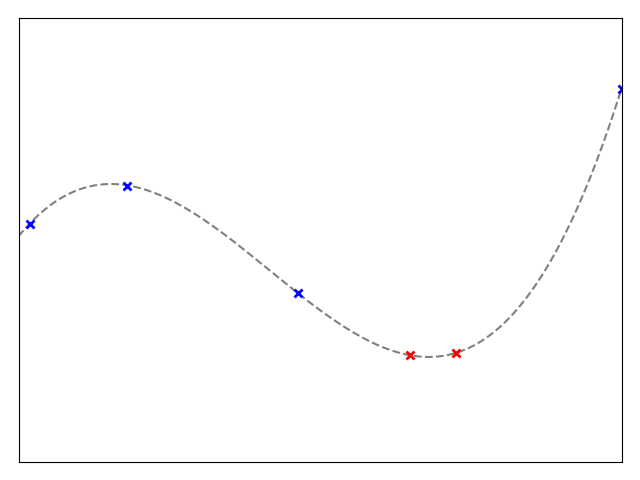
\includegraphics[width=0.6\textwidth]{w07_hpo_grey_box/images/tpe/tpeiter_2_observations.png}


\end{frame}
%-----------------------------------------------------------------------
%-----------------------------------------------------------------------
\begin{frame}[c]{Optimization with Tree-Parzen Estimator}

\centering
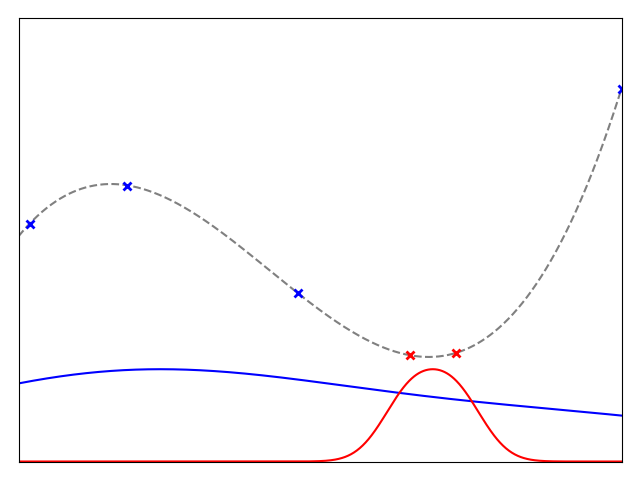
\includegraphics[width=0.6\textwidth]{w07_hpo_grey_box/images/tpe/tpeiter_2_pdfs.png}


\end{frame}
%-----------------------------------------------------------------------
%-----------------------------------------------------------------------
\begin{frame}[c]{Optimization with Tree-Parzen Estimator}

\centering
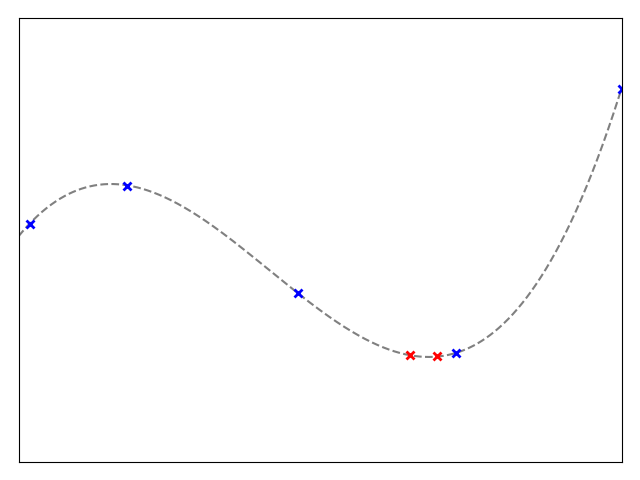
\includegraphics[width=0.6\textwidth]{w07_hpo_grey_box/images/tpe/tpeiter_3_observations.png}


\end{frame}
%-----------------------------------------------------------------------
%-----------------------------------------------------------------------
\begin{frame}[c]{Optimization with Tree-Parzen Estimator}

\centering
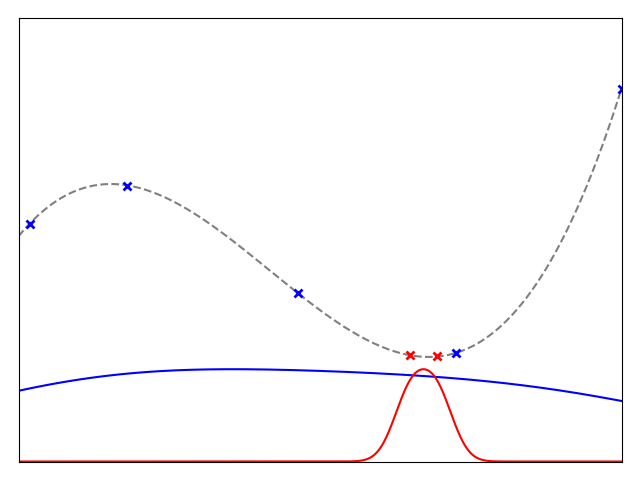
\includegraphics[width=0.6\textwidth]{w07_hpo_grey_box/images/tpe/tpeiter_3_pdfs.png}


\end{frame}
%-----------------------------------------------------------------------
%-----------------------------------------------------------------------
\begin{frame}[c]{Optimization with Tree-Parzen Estimator}


Remarks:

\begin{itemize}
	\item TPE models $p(\conf | \boobs)$
	\begin{itemize}
		\item we can multiply it with a prior to add expert knowledge
	\end{itemize}
	\smallskip
	\pause
	\item Performance of TPE depends on:
	\begin{itemize}
		\item setting of $\gamma$ to trade-off exploration and exploitation
		\item bandwidth of the KDEs 
	\end{itemize}
	\pause
	\smallskip
	\item optimizing $l(\conf)/g(\conf)$ is equivalent to optimizing \emph{expected improvement} as acquisition function in Bayesian Optimization
	\pause
	\smallskip
	\item successful tool implementing TPE is HyperOpt
\end{itemize}

\end{frame}
%-----------------------------------------------------------------------
%-----------------------------------------------------------------------
\begin{frame}[c]{Optimization with Tree-Parzen Estimator: Summary}
\begin{columns}[T] % align columns
\begin{column}{.48\textwidth}


    \begin{block}{Advantages}
    \begin{itemize}
    	\item Efficient $O(N*d)$
    	\pause
    	\item Parallelizable
    	\pause
    	\item Robust
    	\pause
    	\item Deal with complex search spaces with priors
    	\pause
    \end{itemize}
    \end{block}
\pause
\end{column}%

\hfill%

\begin{column}{.48\textwidth}

    \begin{block}{Disadvantages}
    \begin{itemize}
    	\item Less sample-efficient than GPs
    \end{itemize}
\end{block}

\end{column}
\end{columns}   

\end{frame}
%-----------------------------------------------------------------------
%-----------------------------------------------------------------------
